\documentclass[a4paper,cs4size,adobefonts,cm-default,no-math]{ctexart}

\usepackage[
     left=2.7cm,
     right=2.7cm,
     top=3.5cm,
     bottom=2.6cm]{geometry}
%-------------------------------------------------------------------------
\usepackage{fancyhdr}
\pagestyle{fancy}

\fancyhf{}
\fancyhead[EC,OC]{\zihao{-5}北京化工大学毕业设计(论文)外文文献翻译}
\fancyfoot[C]{\thepage}
\renewcommand{\headrulewidth}{0pt}
\renewcommand{\footrulewidth}{0pt}

\newCJKfontfamily[shusong]\shusong{方正书宋_GBK}
\newCJKfontfamily[biaosong]\biaosong{方正小标宋_GBK}


%-------------------------------------------------------------------------
\CTEXsetup[format+=\zihao{-3}]{chapter}
\CTEXsetup[format+=\zihao{-3}]{section}
\CTEXsetup[format+=\zihao{-4}]{subsection}
\CTEXsetup[format+=\zihao{-4}]{subsubsection}
%-------------------------------------------------------------------------

\usepackage{mdwlist}
\usepackage{sistyle}

\usepackage{longtable}
\usepackage{booktabs}
\usepackage{tabularx}
\usepackage{dcolumn}
\usepackage[tbtags]{amsmath}
% \usepackage{pxfonts}
% \usepackage[T1]{fontenc}
% \usepackage{mathptmx}
% \usepackage[T1]{fontenc}
% \usepackage{tgtermes}
% \usepackage[T1]{fontenc}
\usepackage[T1]{fontenc}
%上标定义-----------------------------------------------------------------------------
\makeatletter
\def\@cite#1#2{\textsuperscript{[{#1\if@tempswa , #2\fi}]}}
\newcommand*{\rom}[1]{\expandafter\@slowromancap\romannumeral #1@}
\newcommand{\dif}{\mathrm{d}}
\makeatother
\newtheorem{Definition}{定义}[section]
\newtheorem{Theorem}[Definition]{定理}
%------------------------------------------------------------------------------------
\newenvironment{paralist}{\begin{quote}	\begin{description}\setlength{\itemsep}{0em}}
			 {\end{description}\end{quote}\par}

			 
			 
\newcommand*{\me}{\ensuremath{\mathrm{e}}}    %自然对数的底
\newcommand*{\mi}{\ensuremath{\mathrm{i}}}        %虚数单位
%\newcommand*{\dif}{\ensuremath{\mathrm{d}}}        %微分算子

%\setmainfont{Computer Modern}
%\setsansfont[Scale=MatchLowercase]{Latin Modern Sans}
%\setmonofont[Scale=MatchLowercase]{Inconsolata}


\begin{document}
\setlength{\baselineskip}{22pt}
\begin{titlepage}
\thispagestyle{empty}
\newcommand{\HRule}{\rule{\linewidth}{0.5mm}} % Defines a new command for the horizontal lines, change thickness here

\center % Center everything on the page
 
%----------------------------------------------------------------------------------------
%	HEADING SECTIONS
%----------------------------------------------------------------------------------------

% \textsc{\Large 北京化工大学}\\[1.5cm] % Name of your university/college
\vspace*{1.2cm}
\textsc{\zihao{-3} 北京化工大学本科毕业设计(论文)}\\[2.8cm] % Major heading such as course name
% \textsc{\large Minor Heading}\\[0.5cm] % Minor heading such as course title

%----------------------------------------------------------------------------------------
%	TITLE SECTION
%----------------------------------------------------------------------------------------

\vspace*{1.2cm}
{\heiti \zihao{2}微生物土壤运移模型的求解及仿真软件编制 \biaosong\zihao{2} \\ [0.8cm]外文文献翻译}\\[1cm] % Title of your document
\vspace*{1.2cm}
 
%----------------------------------------------------------------------------------------
%	AUTHOR SECTION
%----------------------------------------------------------------------------------------

% \begin{minipage}{0.4\textwidth}
% \begin{flushleft} \large
% \emph{作者:}\\
% John \textsc{Smith} % Your name
% \end{flushleft}
% \end{minipage}
% ~
% \begin{minipage}{0.4\textwidth}
% \begin{flushright} \large
% \emph{Supervisor:} \\
% Dr. James \textsc{Smith} % Supervisor's Name
% \end{flushright}
% \end{minipage}\\[4cm]
{\kaishu\large
陆秋文\\
北京化工大学生命科学与技术学院\\[0.5cm]}
指导教师\\
{\large\kaishu 周\quad 延}
% If you don't want a supervisor, uncomment the two lines below and remove the section above
%\Large \emph{Author:}\\
%John \textsc{Smith}\\[3cm] % Your name

%----------------------------------------------------------------------------------------
%	DATE SECTION
%----------------------------------------------------------------------------------------
\vfill
% {\large 北京化工大学}\\
{\large 二〇一三年六月三日}\\[0.5cm] % Date, change the \today to a set date if you want to be precise

%----------------------------------------------------------------------------------------
%	LOGO SECTION
%----------------------------------------------------------------------------------------

%\includegraphics{Logo}\\[1cm] % Include a department/university logo - this will require the graphicx package
 
%----------------------------------------------------------------------------------------

 % Fill the rest of the page with whitespace
\end{titlepage}

\title{\kaishu 基于格林函数定律的用于对流扩散反应方程的非标准有限差分格式
      \footnote{英文标题:Nonstandard finite difference schemes based on Green's function
formulations for reaction--diffusion--convection systems,发表在\textit{Chemical Engineering Science}.}}
\author{Eliseo Hernandez-Martinez \and Hector Puebla \and Francisco Valdes-Parada \and Jose Alvarez-Ramirez}
\date{}
\maketitle
\begin{abstract}
非标准有限差分格式可以提高解的准确性,也可以减少相对于传统差分格式的计算量.然而,这些差分格式的建立
依赖于解析解的求解和\textit{Ad hoc}规则.在这篇论文中,我们得到了一种基于格林函数的对流扩散反应方程的NSFD格式.NFSD格式
定理的推导分为三个阶段.在第一阶段,原始的边值问题被分解为N个子域,在第二阶段,对于每一个子域,我们得到其基于格林函数的积分定律.
最后,通过积分法则确定积分结果.\par
自然地,基于格林函数的NFSD差分格式包含了对于边界节点的离散化估计.同时,它也表现出相对于标准FD差分格式较小误差的
$O(h^2)$阶次的估计误差.作为例子,我们研究了催化过程的偏微分方程模型和反应器模型的数值模拟,采用了NFSD格式
与标准有限差分法准确性和性能的差别.
\end{abstract}
\thispagestyle{empty}
\newpage
\section{介绍}
在很多科学领域,包括物理学、生物学、环境工程和化学工程中,都大量存在对流扩散过程,化学反应过程系统也是如此.众所周知,找到一个非线性
偏微分方程的解析解是困难的,甚至,这样的解析解是不存在的.这样,我们就要考虑采用数值方法来解偏微分方程.对于对流扩散反应系统(RDC)来说,
有一些特别的方法已经被报道了.例如,~Alhumaizi等人发表了一个RDC系统的差分法和有限元法的分析,~Coimbra等人建立了一种移动有限元法来解
时变的RDC问题.~Hernadez-Martinez等人推导了一种基于格林函数的积分法来求解Danckwerts型边界条件的RDC系统.由于解的稳定性、有效性强,
易于计算机编程实现,有限差分法(FD)已经广泛地用于解RDC--PDE问题.但众所周知,微分运算的离散对截断误差高度敏感.另外,连续系统离散化过程中
不合适的附加参数可能会导致结果的不稳定.\par
在本文中,我们先简短地介绍一维对流扩散反应方程模型的格林函数的推导过程,然后,我们介绍经典的FD差分格式.之后,推导基于格林函数的
NSFD格式.最后,对本文的工作进行总结.
\section{对流扩散反应系统的格林函数定理}\label{sec:2}
在这一节中,我们推导基于格林函数的用于解常规边界条件的RDC模型的积分法.\par
\subsection{一维对流扩散反应模型}
通常的PDE模型可以描述为
\begin{equation}\label{eq:1}
 \dfrac{\partial u(x,t)}{\partial t}=\dfrac{\partial^2 u(x,t)}{\partial x^2}-Pe\dfrac{\partial u(x,t)}{\partial x}
 -R(u(x,t)),\qquad x\in[a,b] 
\end{equation}
初始条件
\begin{equation}\label{eq:2}
 u(0,x)=u_0(x)
\end{equation}
常规边界条件
\begin{equation}\label{eq:3}
\begin{aligned}
 \alpha_a\dfrac{\partial u(a,t)}{\partial x}+\beta_a u(a,t)+\gamma_a=&0 \\
 \alpha_b\dfrac{\partial u(b,t)}{\partial x}+\beta_b u(b,t)+\gamma_b=&0
\end{aligned}
\end{equation}
其中,~$\alpha_i$,$\beta_i$为常数,~$Pe$是佩克莱数(Peclet Number),~用于表示对流和扩散过程的关系.\par
方程~\ref{eq:1}~和边界条件~\ref{eq:2}~构成了一个完整的用于描述RDC系统的方程组.这个方程组能够描述工程中大量
的分布参数系统,例如管式反应器、污染物运移问题、生物种群的相互作用、晶体单元和催化剂颗粒的传递现象等.
\subsection{基于格林函数的积分形式}
为了推导方程~\ref{eq:1}~的积分形式,我们采用Hernandez-Martinez的方法,设积分因子$\sigma=\exp(-Pex)$,我们得到方程~\ref{eq:1}~的共轭形式为
\begin{equation}\label{eq:4}
 \dfrac{\partial}{\partial x}\left[\exp(-Pex)\dfrac{\partial u(x,t)}{\partial x}\right]=\exp(-Pex)\Psi(x,t)
\end{equation}
其中,~$\Psi(x,t)=(\partial u(x,t)/\partial t)+R(u(x,t))$.定义
\begin{equation*}
 L=\dfrac{\partial}{\partial x}\left[\exp(-Pex)\dfrac{\partial}{\partial x}\right]
\end{equation*}
作为式~\ref{eq:4}~的微分算子,引入格林函数$G(z,x)$,部分积分,式~\ref{eq:4}~变为
\begin{equation}\label{eq:6}
\begin{split}
  \int_a^b\dfrac{G(z,x)}{\exp(Pez)}\Psi(x,t)\dif z=&\exp(-Pez)\left[G(z,x)\dfrac{\partial u(z,t)}{\partial z}
 -\dfrac{\partial G(z,x)}{\partial z}u(z,t)\right]_a^b\\&+\int_a^b u(z,t)L^*G(z,x)\dif z
\end{split}
\end{equation}\par
在另一方面,~$G(z,x)$的边值条件问题由下式给出,即
\begin{equation}
 L^*G(z,x)=\delta(x-z)
\end{equation}
和边界条件
\begin{equation}\label{eq:7}
 \begin{aligned}
  \alpha_a\dfrac{\partial G(a,x)}{\partial x}+\beta_a G(a,x)+\gamma_a=&0 \\
  \alpha_b\dfrac{\partial G(b,x)}{\partial x}+\beta_b G(b,x)+\gamma_b=&0
 \end{aligned}
\end{equation}
其中,~$\delta(z-x)$是狄拉克函数,其滤波特性可以表为
\begin{equation*}
 \int_a^b u(z,t)\delta(z-x)\dif z=u(x,t)
\end{equation*}
我们利用这个特性来计算边界条件~\ref{eq:7}~,得
\begin{equation}\label{eq:8}
 \begin{split}
  u(x,t)=&\exp(-Pea)\dfrac{\partial G(a,x)}{\partial z}\dfrac{\gamma_a}{\beta_a}-\exp(-Peb)\dfrac{G(b,x)}
  {\partial z}\dfrac{\gamma_b}{\beta_b}\\
  &+\int_a^b\dfrac{G(z,x)}{\exp(Pez)}\Psi(z,t)\dif z
 \end{split}
\end{equation}\par
方程~\ref{eq:8}~是方程~\ref{eq:1}~的积分形式,其解需要相应的格林函数$G(z,x)$.
\subsection{格林函数的求解}
式~\ref{eq:6}~的边界条件由式~\ref{eq:7}~给出,其积分形式为
\begin{equation}\label{eq:9}
 G(z,x)=\dfrac{1}{Pe}
 \begin{cases}
 C_1\left[\exp(Pez)-\exp(Pea)\left(1+\dfrac{\alpha_a}{\beta_a}Pe\right)\right] & z<x \\[1.2em]
 C_3\left[\exp(Pez)-\exp(Peb)\left(1+\dfrac{\alpha_b}{\beta_b}Pe\right)\right] & z\geq x 
 \end{cases}
\end{equation}\par
计算常数$C_1$和$C_3$需要额外的两个条件.第一个条件由函数$u(x,t)$在$z=x$处是连续的得来,即$G(x^+,x)=G(x^-,x)$.
第二个条件方程~\ref{eq:6}~的积分形式得到,即下式
\begin{equation*}
 \left.\dfrac{\partial G(z,x)}{\partial z}\right|_{z=x^+}-\left.\dfrac{\partial G(z,x)}{\partial z}\right|_{z=x^-}
 =\exp(Pex)
\end{equation*}
方程~\ref{eq:9}~变为
\begin{equation}\label{eq:10}
 G(z,x)=\dfrac{1}{G^*}
         \begin{cases}
         \left[\exp(Pez)-\exp(Pea)k_a\right]\left[\exp(Pex)-\exp(Peb)k_b\right] & z<x \\
         \left[\exp(Pez)-\exp(Pea)k_b\right]\left[\exp(Pex)-\exp(Peb)k_a\right] & z\geq x
         \end{cases}
\end{equation}
其中,
\begin{equation*}
 G^*=Pe[\exp(Peb)k_b-\exp(Pea)k_a],\qquad k_a=1+\dfrac{\alpha_a}{\beta_a}Pe
\end{equation*}\par
一般地,格林函数~\ref{eq:10}~与方程~\ref{eq:8}~得到了由式~\ref{eq:1}~给出的RDC--PDE问题的积分形式.根据参数$\alpha_i$、
$\beta_i$、$\gamma_i$,~得到不同边界条件下的格林函数是很有可能的(例如:Dirichlet,Neumman,Robin边界条件).
\section{数值格式}
在这一节中,我们论述基于格林函数积分形式的NSFD差分格式的推导.同时,我们也讨论目标NSFD格式的结构,简要地介绍经典的有限差分格式.
\subsection{经典的有限差分格式}
在传统的有限差分格式中,对于RDC模型,大部分的运算可以采用多种方式进行离散.例如,对于一个等距离分布的网格$X_{N+1}=x_a,x_1,\cdots,x_N,x_b$
,其中,~$x_a=a$,$x_b=b$,$x_i-x_{i-1}=h$,并且$u_i(t)=u(x_i,t)$.我们可以从式~\ref{eq:1}~的一个半离散的形式中得出
\begin{equation}\label{eq:11}
 \dfrac{\dif u_i(t)}{\dif t}=\dfrac{(1+\frac{1}{2}Peh)u_{i-1}(t)-2u_i+(1-\frac{1}{2}Peh)u_{i+1}(t)}{h^2}-R(u_i(t))
\end{equation}
其中,$i=1,2,\cdots,N$.空间算子采用二阶中心差分格式来进行估计.对于对流过程,也可以采用向前近似或向后近似来获得下面的差分格式
\begin{itemize}
 \item 向前差分格式
 \begin{equation}\label{eq:12}
  \dfrac{\dif u_i(t)}{\dif t}=\dfrac{u_{i-1}-(2-Peh)2u_i(t)+(1-Peh)u_{i+1}(t)}{h^2}-R(u_i(t))
 \end{equation}
 \item 向后差分格式
 \begin{equation}\label{eq:13}
  \dfrac{\dif u_i(t)}{\dif t}=\dfrac{(1+Peh)u_{i-1}(t)-(2+Peh)u_i(t)+u_{i+1}}{h^2}-R(u_i(t))
 \end{equation}
\end{itemize}\par
要完成空间的离散化,引入边界条件是必要的.孤立节点和拓展网格典型地被用在标准有限差分法的PDE系统的边界条件的离散化.
虽然这些形式是很容易实现的,但是我们仍假设它们是存在的.这些假设可能会带来弱数值解来描述非物理现象.因此,我们在推导中
要避开这些孤立节点,为此,一阶的有限差分格式就很常用了.
\subsection{基于格林函数公式的NSFD}
为了推导式~\ref{eq:1}--\ref{eq:3}~的基于格林函数公式的NSFD格式,我们采用Alvarez-Ramirez等人发表的方法.对于一个等距离分布的网格
,我们考虑一个重叠的区间$D_i=[x_{i-1},x_{i+1}]$,~$i=1,\cdots,N$.~然后,我们得到下面一组微分方程.
\begin{equation}\label{eq:14}
 \begin{aligned}
  Lu(x,t)&=\Psi(x,t),x\in D_1,\alpha_a\dfrac{\partial u(x_a,t)}{\partial x}+\beta_a u(x_a,t)+\gamma_a=0,u(x_2,t)=u_2(t)\\
  Lu(x,t)&=\Psi(x,t),x\in D_i,u(x_{i-1},t)=u_{i-1}(t),u(x_{i+1},t)=u_{i+1}(t),i=2,\cdots,N-1 \\
  Lu(x,t)&=\Psi(x,t),x\in D_N,u(x_{N-1},t)=u_{N-1}(t),\alpha_b\dfrac{\partial u(x_b,t)}{\partial x}
          +\beta_b u(x_b,t)+\gamma_b=0
 \end{aligned}
\end{equation}\par
为了说明这个过程,我们考虑方程~\ref{eq:14}~具有一个Dirichlet型的边界条件.与第~\ref{sec:2}~节中的结果一致,方程~\ref{eq:14}~的积分形式为
\begin{equation}\label{eq:15}
\begin{split}
 u(x,t)=&\exp(Pex_{i-1})\dfrac{\partial G_i(x_{i-1},x)}{\partial z}u_{i-1}(t)-\exp(Pex_{i+1})\dfrac{\partial
 G_i(x_{i+1},x)}{\partial z}u_{i+1}\\[0.6em]
 &+\int_{x_{i-1}}^{x_{i+1}}\dfrac{G_i(z,x)}{\exp(Pez)}\Psi(z,t)\dif t
\end{split}
\end{equation}
考虑方程~\ref{eq:10}~的Dirichelet型边界条件($\alpha_a=\alpha_b=0,\beta_a=\beta_b=0$),相应的格林函数为
\begin{equation}
 G_i(z,x)=\dfrac{1}{G^*}
 \begin{cases}
  [\exp(Pex)-\exp(Pex_{i+1})][\exp(Pez)-\exp(Pex_{i+1})] & z<x \\
  [\exp(Pez)-\exp(Pex_{i+1})][\exp(Pex)-\exp(Pex_{i+1})] & z\geq x 
 \end{cases}
\end{equation}
其中,~$G^*=Pe[\exp(Pex_{i+1})-\exp(Pex_{i-1})]$.方程~\ref{eq:15}~在相应的子区间$D_i$内点$x_i$的近似值可以表示为
\begin{equation}\label{eq:17}
\begin{split}
 u_i(t)=&-\dfrac{[\exp(Pex_i)-\exp(Pex_{i-1})]}{\exp(Pex_{i+1})-\exp(Pex_{i-1})}u_{i+1}(t)
        -\dfrac{[\exp(Pex_{i+1})-\exp(Pex_i)]}{\exp(Pex_{i+1})-\exp(Pe_{i-1})}u_{i-1}(t) \\[0.5\baselineskip]
        &+\int_{x_{i-1}}^{x_{i+1}}\dfrac{G_i(z,x)}{\exp(Pez)}\Psi(z,t)\dif z
\end{split}
\end{equation}\par
为了得到式~\ref{eq:17}~积分的近似值,我们采用等距三点的梯形规则,即
\begin{multline}\label{eq:18}
 \int_{x_{i-1}}^{x_{i+1}}\dfrac{G_i(z,x)}{\exp(Pez)}\Psi(z,t)\dif z \approx\\
 -\dfrac{[\exp(Pex_i)-\exp(Pex_{i-1})][\exp(Pex_{i+1})-\exp(Pex_i)]}{Peh\exp(Pex_i)[\exp(Pex_{i+1})-\exp(Pex_{i-1})]}
 h^2\Psi_i(t)
\end{multline}
将式~\ref{eq:18}~代入式~\ref{eq:17}~中,得
\begin{equation*}
 \begin{split}
  u_i(t)=&-\dfrac{[\exp(Pex_i)-\exp(Pex_{i-1})]}{\exp(Pex_{i+1})-\exp(Pex_{i-1})}u_{i+1}(t)\\[0.5\baselineskip]
        &-\dfrac{[\exp(Pex_{i+1})-\exp(Pex_i)]}{\exp(Pex_{i+1})-\exp(Pe_{i-1})}u_{i-1}(t) \\[0.5\baselineskip]
        &-\dfrac{[\exp(Pex_i)-\exp(Pex_{i-1})][\exp(Pex_{i+1})-\exp(Pex_i)]}{Peh\exp(Pex_i)[\exp(Pex_{i+1})-\exp(Pex_{i-1})]}
 h^2\Psi_i(t)
 \end{split}
\end{equation*}
或
\begin{equation}\label{eq:19}
 a_i u_{i-1}(t)-b_iu_i(t)+c_iu_{i+1}(t)=\Psi_i(t)
\end{equation}
对于子区间$D_1$和$D_N$,重复方程~\ref{eq:15}~到~\ref{eq:19}~的过程,我们得到下面的一组方程
\begin{equation}\label{eq:20}
 \begin{aligned}
  \dfrac{\dif u_1(t)}{\dif t} &=a_1\dfrac{\gamma_a}{\gamma_b}-b_1u_1(t)+c_1u_2(t)-R(u_1(t))\\
  \dfrac{\dif u_i(t)}{\dif t} &=a_iu_{i-1}(t)-b_iu_i(t)-c_iu_{i+1}(t)-R(u_i(t))\\
  \dfrac{\dif u_N(t)}{\dif t} &=a_Nu_{N-1}(t)-b_Nu_N(t)-c_N\dfrac{\gamma_b}{\beta_b}-R(u_N(t))
 \end{aligned}
\end{equation}
离散化参数为
\begin{align*}
 a_1 &=\dfrac{Pe\xi_1}{h(C_1\xi_a-\xi_1)},& b_1&=\dfrac{\xi_2-\xi_a k_a}{\xi_1-\xi_2}a_1, & c_1&=\dfrac{\xi_1-\xi_a k_a}{\xi_2-\xi_1}a_1 \\
 a_i &=\dfrac{Pe\xi_i}{h(\xi_i-i_{i-1})},& b_i&=\dfrac{\xi_{i+1}-\xi_{i-1}}{\xi_{i+1}-\xi_i}a_i, & c_i &=\dfrac{Pe\xi_i}{h(\xi_{i+1}-\xi_{i})}\\
 a_N &=\dfrac{\xi_N-\xi_a k_b}{\xi_N-\xi_{N-1}}c_N,& b_N&=\dfrac{\xi_{N-1}-\xi_b k_n}{\xi_N-\xi_{N-1}}c_N,& c_N&=\dfrac{Pe\xi_N}{h(\xi_N-C_2\xi_b)}
\end{align*}
其中,~$\xi_i=\exp(Pex_i)$,$C_1=1+\frac{3}{2}(\alpha_a/\beta_a)Pe$,$C_2=1+\frac{3}{2}(\alpha_b/\beta_b)$.\par
\vspace*{0.4em}
在推导基于格林函数的NSFD结构,有几点需要注意如下:
\begin{itemize}
 \item 权重参数$a_i$,$b_i$,$c_i$~($i=1,\cdots,N$)是$h$的函数.根据Mickens(1989)给出的定义,方程~\ref{eq:20}~
 给出的系统可以被看作带普通边界条件的RDC系统的NSDF差分格式.
 \item 传统上推导传递反应过程的偏微分方程的NSFD格式使用的是子方程法.使用有限差分和梯形规则来得到子方程结果.最后,组合成
 离散方程.在上面的推导过程中,我们看到不使用经验规则,也可以由格林函数推导出NSFD格式.参数~$a_i$,$b_i$,$c_i$~只由格林函数的
 性质决定.
 \item 方程~\ref{eq:11}~给出的标准有限差分格式是基于格林函数的NSFD格式的特例.为了证明这一点,在式~\ref{eq:20}~中将$a_i$
 乘上$\xi_{i-1/2}/\xi_{i-1/2}$~,得到
 \begin{equation*}
  a_i=\dfrac{Pe\exp(\frac{1}{2}Peh)}{h(\exp(\frac{1}{2}Peh)-\exp(-\frac{1}{2}Peh))}
 \end{equation*}
考虑指数函数泰勒展开式的前两项
\begin{equation*}
 a_i \approx \dfrac{1+\frac{1}{2}Peh}{h^2}
\end{equation*}
相应地用$\xi_i/\xi_i$和$\xi_{i-1/2}/\xi_{i-1/2}$代替$b_i$和$c_i$~,得到$b_i\approx2/h^2$和$c_i\approx(1-\frac{1}{2}
Peh)/h^2$~.在这样的形式下,重新得到方程~\ref{eq:11}~给出的中心差分格式是有可能的.
\item 式~\ref{eq:20}~给出的方程组是常规(一维)对流传递方程的NSFD差分格式.在这种情况下,得到对流反应方程或对流扩散方程的特例
是有可能的.例如,我们考虑令$Pe\rightarrow0$~,方程~\ref{eq:20}~的权重参数就变为
\begin{align*}
 a_1 &= \dfrac{h}{h^2\left(h-\dfrac{3}{2}\dfrac{\alpha_a}{\beta_a}\right)}, 
 & b_1&=\dfrac{2h-\dfrac{\alpha_a}{\beta_a}}{h^2\left(h-\dfrac{3}{2}\dfrac{\alpha_a}{\beta_a}\right)}, 
 & c_1 &=\dfrac{h-\dfrac{\alpha_a}{\beta_a}}{h^2\left(h-\dfrac{3}{2}\dfrac{\alpha_a}{\beta_a}\right)},\\
 a_i &=\dfrac{1}{h^2}, & b_i&=\dfrac{2}{h^2}, & c_i&=\dfrac{1}{h^2}, \\
 a_N &=\dfrac{h-\dfrac{\alpha_b}{\beta_b}}{h^2\left(h+\dfrac{3}{2}\dfrac{\alpha_b}{\beta_b}\right)}, &
 b_N &=\dfrac{2h-\dfrac{\alpha_b}{\beta_b}}{h^2\left(h+\dfrac{3}{2}\dfrac{\alpha_b}{\beta_b}\right)}, &
 c_N &=-\dfrac{h}{h^2\left(h+\dfrac{3}{2}\dfrac{\alpha_a}{\beta_b}\right)},
\end{align*}
得到常规边界条件下的对流反应方程的NSFD差分格式.我们需要指出,在Dirichlet型边界条件下,$a_i$,$b_i$,$c_i$~的值与经典FD差分格式
一致.如果我们考虑混合边界条件($\partial u(0,t)/\partial t=1$并且$u(1,t)=1$),在边界上的权重参数为$b_1=c_1=\frac{2}{3}$,
$a_1=c_N=0$,$a_N=1$,$b_N=2$.Alvarez-Ramirez等人发表了这样的结论:广泛的数值模拟证明权重因子3/2对于减少FD差分格式的近似误差有着重要的作用.我们注意到,3/2这样
的一个数值是由边界条件的参数值得来的.这说明了在不同类型的边界条件下,目标数值差分格式比传统的FD差分格式要好.
\item 在积分离散化过程中使用梯形规则的作用是得到因数3/2,从而得到一个二阶的NSFD差分格式.三角形规则的使用去掉了因数3/2,得到了在
边界上的一阶近似.这实现了$O(h)$阶的近似.通过考虑一个更高阶次的积分,我们可以得到NSFD格式的高阶近似.
\item 尽管为了简化论述,我们的分析建立在一维RDC系统上,然而建立NSFD格式可以拓展到二维或三维系统.例如,考虑一个二维RDC模型如下
\begin{equation}\label{eq:21}
 \dfrac{\partial u(x,y,t)}{\partial t}=\dfrac{\partial^2 u(x,y,t)}{\partial x^2}+
                                       \dfrac{\partial^2 u(x,y,t)}{\partial y^2}-
                                       Pe_x\dfrac{\partial^2 u(x,y,t)}{\partial x^2}
                                       -R(u(x,y,t))
\end{equation}
一个得到NSFD差分格式的直接方法是分离空间微分算子.整理式~\ref{eq:21}~,重复方程~\ref{eq:14}--\ref{eq:20}~的步骤,得到以下方程
\begin{equation}\label{eq:22}
 \begin{aligned}
  \dfrac{\partial u_1(y,t)}{\partial t}-\dfrac{\partial^2 u_1(y,t)}{\partial y^2} &=
  a_1\dfrac{\gamma_a}{\beta_a}-b_1 u_1(y,t)+c_1 u_2(y,t)-R(u_1(y,t)) \\
  \dfrac{\partial u_i(y,t)}{\partial t}-\dfrac{\partial^2 u_i(y,t)}{\partial y^2} &=
  a_i u_{i-1}(y,t)-b_i u_{i+1}(y,t)-R(u_i(y,t)) \\
  \dfrac{\partial u_N(y,t)}{\partial t}-\dfrac{\partial^2 u_N(y,t)}{\partial y^2} &=
  a_Nu_{N-1}(y,t)-b_Nu_N(y,t)+c_N\dfrac{\gamma_b}{\beta_b}-R(u_N(y,t))
 \end{aligned}
\end{equation}
最后,对系统~\ref{eq:22}~中的每一个方程进行迭代计算,得到常微分方程组.另外一个选择是采用梯形规则或数值积分的方法进行二维模型的积分.
\item NSFD差分格式的推导过程考虑了Robin型边界条件.依赖于反应过程历史的边界条件可以很容易得到.在空间内的节点的过程也是相同的.
\end{itemize}
\section{数值解}
在这一节中我们来说明基于格林函数的NSFD差分格式得到对流扩散反应方程准确解的能力.在最后,我们考虑两种例子:(i)催化剂微粒和(ii)非等温
管式反应器.为了评价目标数值差分格式的性能,我们分析稳态和动态仿真,并与传统的FD差分格式进行对比.在稳态情况下,离散形式的空间算子可以得到
,非线性代数方程可以通过牛顿——辛普森法来解.对于动态的情况,我们采用直线法来获得空间离散和一组用龙格库塔法得到的原始微分方程的积分形式的方程.\par
我们采用\texttt{AMD Turion(TM) 2 P560}双核处理器,~\texttt{4GB}内存的PC机来得到数值仿真的结果.为了考察NSDF的数值结果的准确度,我们在推导
催化颗粒的算例中得到解析解,并与数值解进行比较.在管式反应器算例中,我们通过\texttt{COMSOL Multiphysics 4.3a}系统得到2000个节点的计算结果
并与我们的数值解进行比较.
\subsection{催化剂颗粒算例}
考虑有线性函数的$R(u(x))=\Psi^2 u(x,t)$的方程~\ref{eq:1}~.这样的一个方程是可以描述催化剂颗粒的对流扩撒反应方程.它的数学模型
由下式给出
\begin{equation}\label{eq:23}
 \dfrac{\partial u(x,t)}{\partial t}=\dfrac{\partial^2 u(x,t)}{\partial x^2}-Pe\dfrac{\partial u(x,t)}{\partial x}
 -\phi^2(x)
\end{equation}
它的初值和边界条件为$u(x,0)=0,u(0,t)=1,u(1,t)=1$.相应地,函数$u(x,t)$代表浓度;$\phi$是Thiele系数,与化学反应的速率和扩散速率有关.
无维度参数$x\in[0,1],t>0$相应地代表空间坐标和时间.为了说明在催化颗粒中的化学反应和传递现象,图~\ref{fig:1}~说明了在不同的$Pe$和$\phi$
时空上的模拟情况.
\begin{figure}
 \centering
 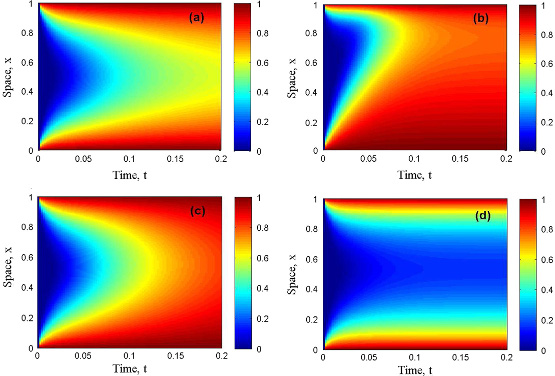
\includegraphics[scale=0.7]{./pic/1.jpg}
 \caption{不同$Pe$和$\phi$催化剂颗粒模型的时空分布模拟情况}\label{fig:1}
\end{figure}
\subsubsection{稳态}
令方程~\ref{eq:23}~中$\partial u(x,t)/\partial t=0$,可以得到一个解析解
\begin{equation}\label{eq:24}
 u(x)=\dfrac{\exp(m_2 x)[\exp(m_1)-1]+\exp(m_1 x)[1-\exp(m_2)]}{\exp(m_1)-\exp(m_2)}
\end{equation}
其中
\begin{equation*}
 m_1=\dfrac{\sqrt{Pe^2+4\phi^2}}{2},\quad m_2=\dfrac{\sqrt{Pe^2-4\phi^2}}{2}
\end{equation*}\par
我们计算最大误差($E_m$)作为单一的指标来表示近似误差,定义为
\begin{equation}\label{eq:25}
 E_m = \max\left|\dfrac{u_e(x_i)-u(x_i)}{u_e(x_i)}\right|
\end{equation}
其中,~$u_e(x_i)$和$u(x_i)$与解析解和在相应点处的近似解有关.\par
在数值模拟上,我们使用向后、中心和向前的差分格式(即方程~\ref{eq:11}--\ref{eq:13}).
以及NSFD差分格式(方程~\ref{eq:20},其中$\alpha_a=\alpha_b=0,\beta_a=\beta_b=1,\gamma_a=\gamma_b=-1$).
这一组代数方程是采用\texttt{MATLAB}库中的Newton-Raphson法求解的.\par
\begin{figure}
\centering
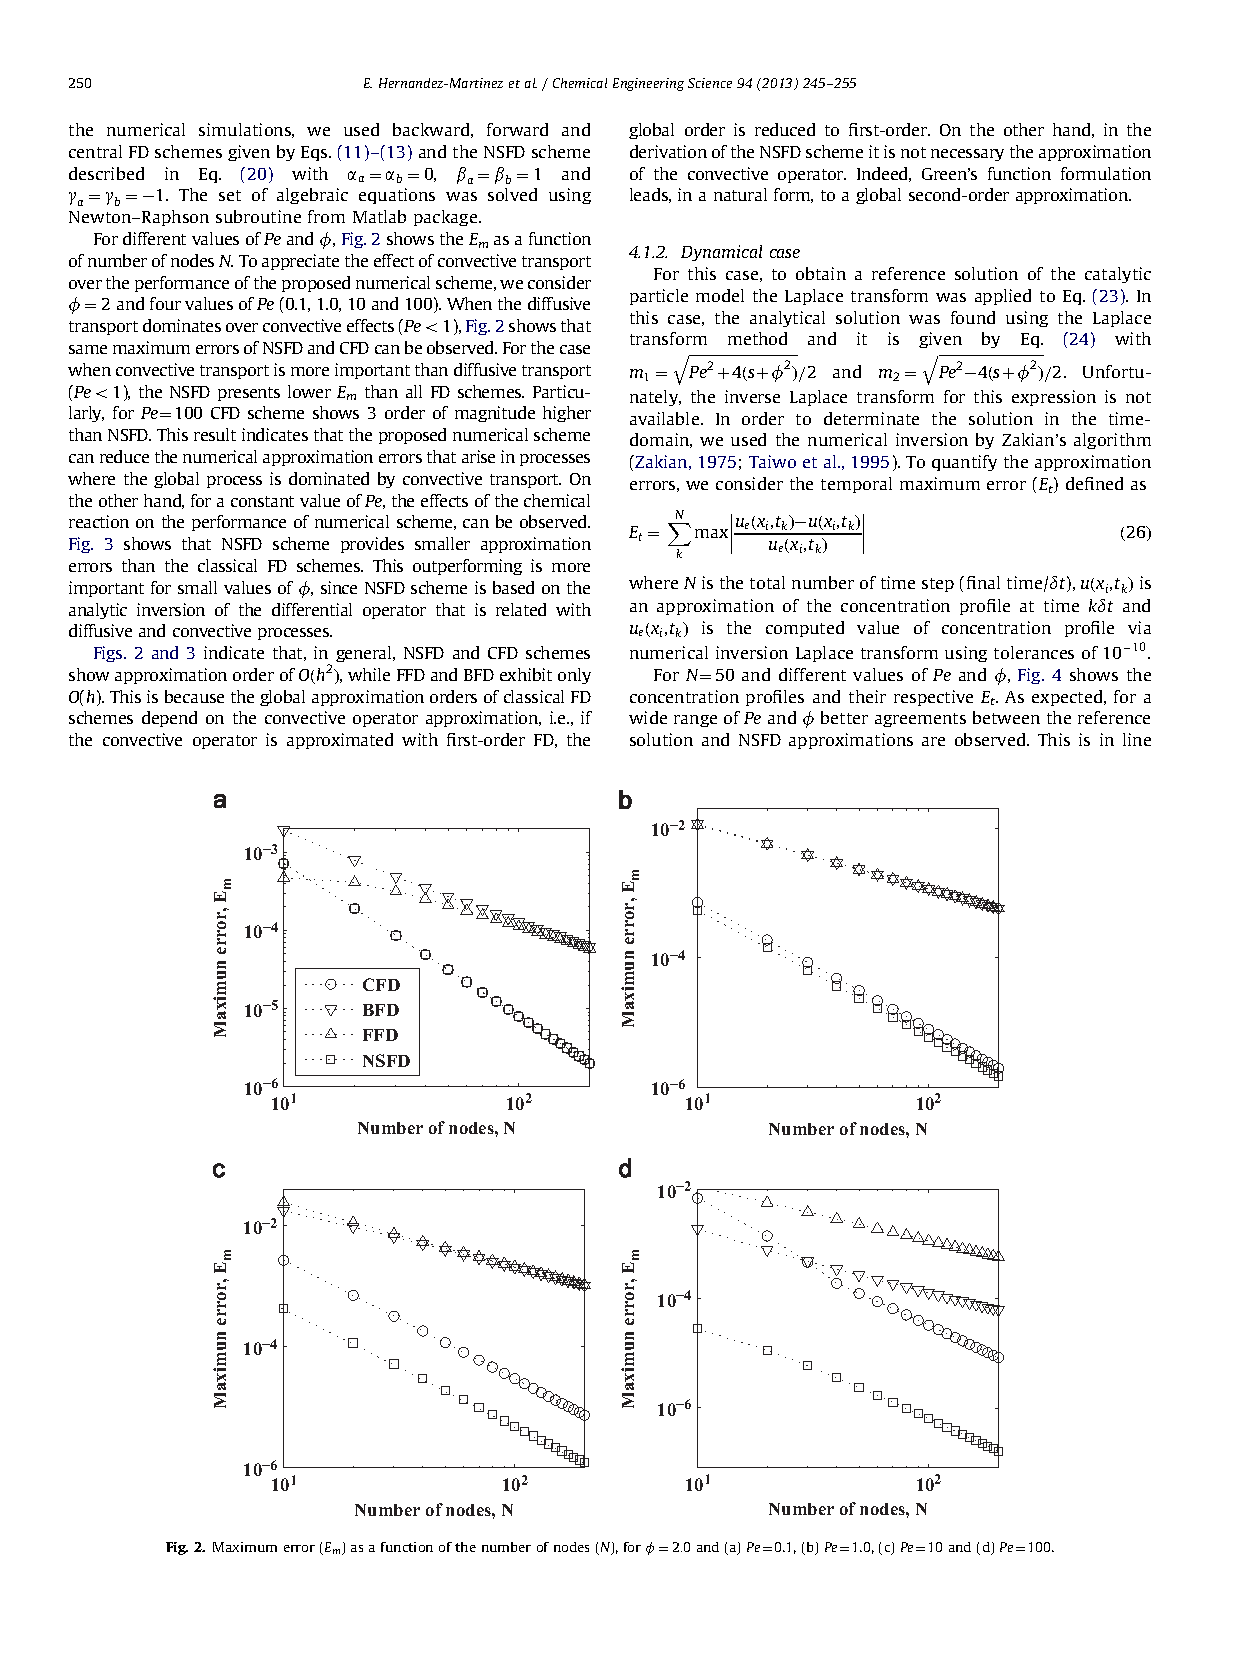
\includegraphics[trim=80 60 80 375,clip]{./pic/f2.pdf}
\caption{节点数($N$)与最大误差($E_m$)的关系}\label{fig:2}
\end{figure}\par
对于不同的$Pe$和$\phi$值,图~\ref{fig:2}~表达了$E_m$和$N$之间的函数关系.为了体现目标差分格式对于对流过程的表现情况,
我们令$\phi=2$和四个$Pe$值.当扩散过程相对于对流过程占优势时,可以观察到图~\ref{fig:2}~中NSFD格式和CFD格式具有相同的
最大误差.在对流过程比扩散过程更为重要的情况下,NSFD差分格式的误差要低于全部的FD格式.特别地,当$Pe=100$时,CFD格式的误差比
NSFD高了三个数量.这个结果说明了我们目标的差分格式能够减少对流过程占有情况下的数值误差.另外一方面,若$Pe$为常数,我们可以观察到
化学反应过程对数值格式的影响.图~\ref{fig:3}~说明了NSFD比经典的FD差分格式具有更小的近似误差.\par
图~\ref{fig:2}~和图~\ref{fig:3}~表示NSFD和CFD差分格式具有$O(h^2)$阶近似,但FFD和BFD差分格式只有$O(h)$阶的近似.这是因为
因为经典FD差分格式的近似误差决定于对流过程的近似误差.如果对流过程采用了一阶的近似,那么全局的借此就会降低到一阶.另一方面,
NSFD格式的推导过程不需要对流过程进行近似,相反地,格林函数本身就会得到二阶的近似精度.
\begin{figure}
\centering
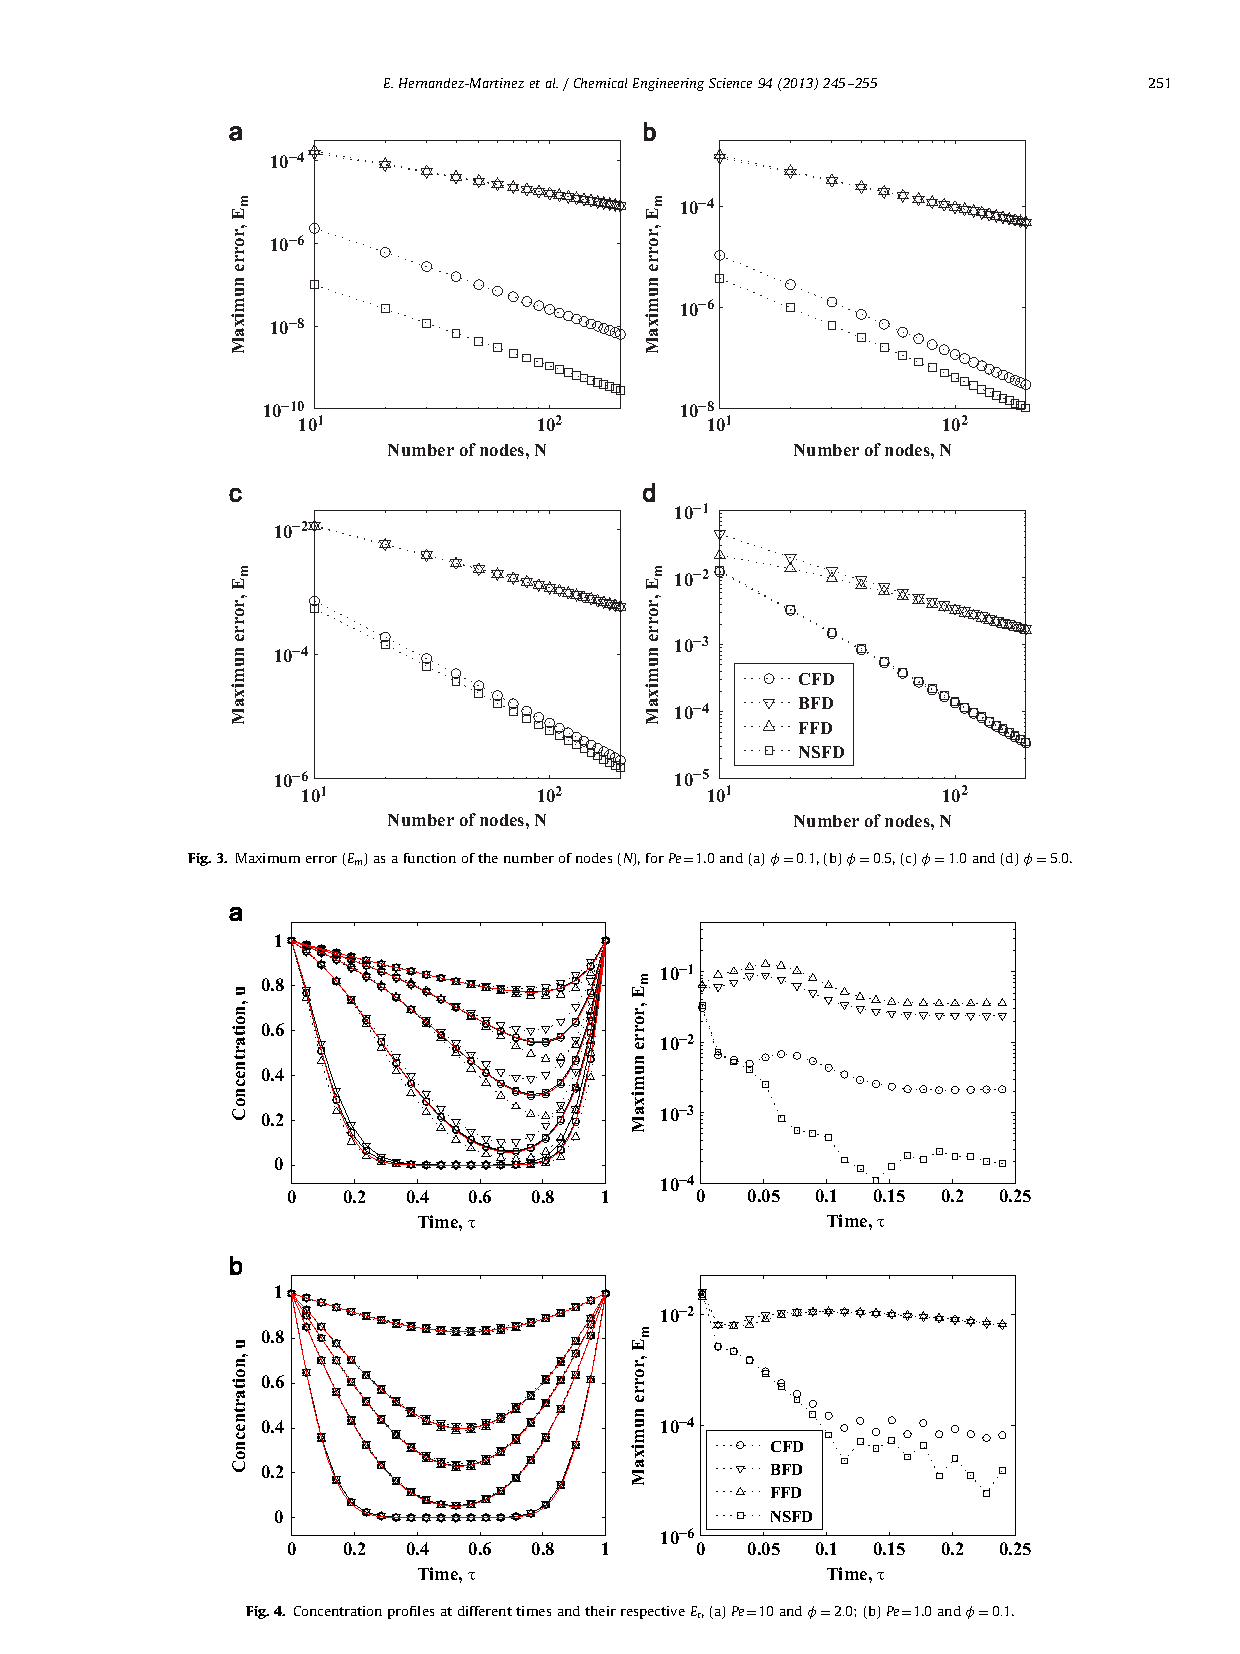
\includegraphics[trim=80 390 80 60,clip]{./pic/f3.pdf}
\caption{当$Pe=1.0$时最大误差($E_m$)与节点数$N$的关系}\label{fig:3}
\end{figure}
\subsubsection{动态}
我们对方程~\ref{eq:23}~进行Laplace变换来得到催化剂颗粒的参考解.在这种情况下,式~\ref{eq:24}~是经Laplace变换后得到的解析解.
其中,
\begin{equation*}
m_1=\dfrac{\sqrt{Pe^2+4(s+\phi^2)}}{2} \qquad m_2=\dfrac{\sqrt{Pe^2-4(s+\phi^2)}}{2}
\end{equation*}
但不幸的是,我们无法得出上式的Laplace逆变换.为了得到最终的解,我们采用了Zakian的数值法来求解它的逆变换.为了确定近似误差,
我们定义时间最大误差为
\begin{equation}
 E_t=\sum_k^N\max\left|\dfrac{u_e(x_i,t_k)-u(x_i,t_k)}{u_e(x_i,t_k)}\right|
\end{equation}
其中,~$N$是时间步的总数(总时间/$\delta t$).~$u(x_i,t_k)$是在$k\delta t$时浓度的近似值.~$u_e(x_i,t_k)$是
通过数值逆Laplace变换后得到的计算值.\par
当$N=50$,~$Pe$和$\phi$取到不同的值时,图~\ref{fig:4}~给出了浓度的变化和相应的$E_t$.可以期望到,我们在参考解和NSFD数值
解中可以观察到更好的参数.例如,对于对立过程主导的条件,~NSFD给出了二阶的误差,相对于CFD格式是较为小的.
\begin{figure}
\centering
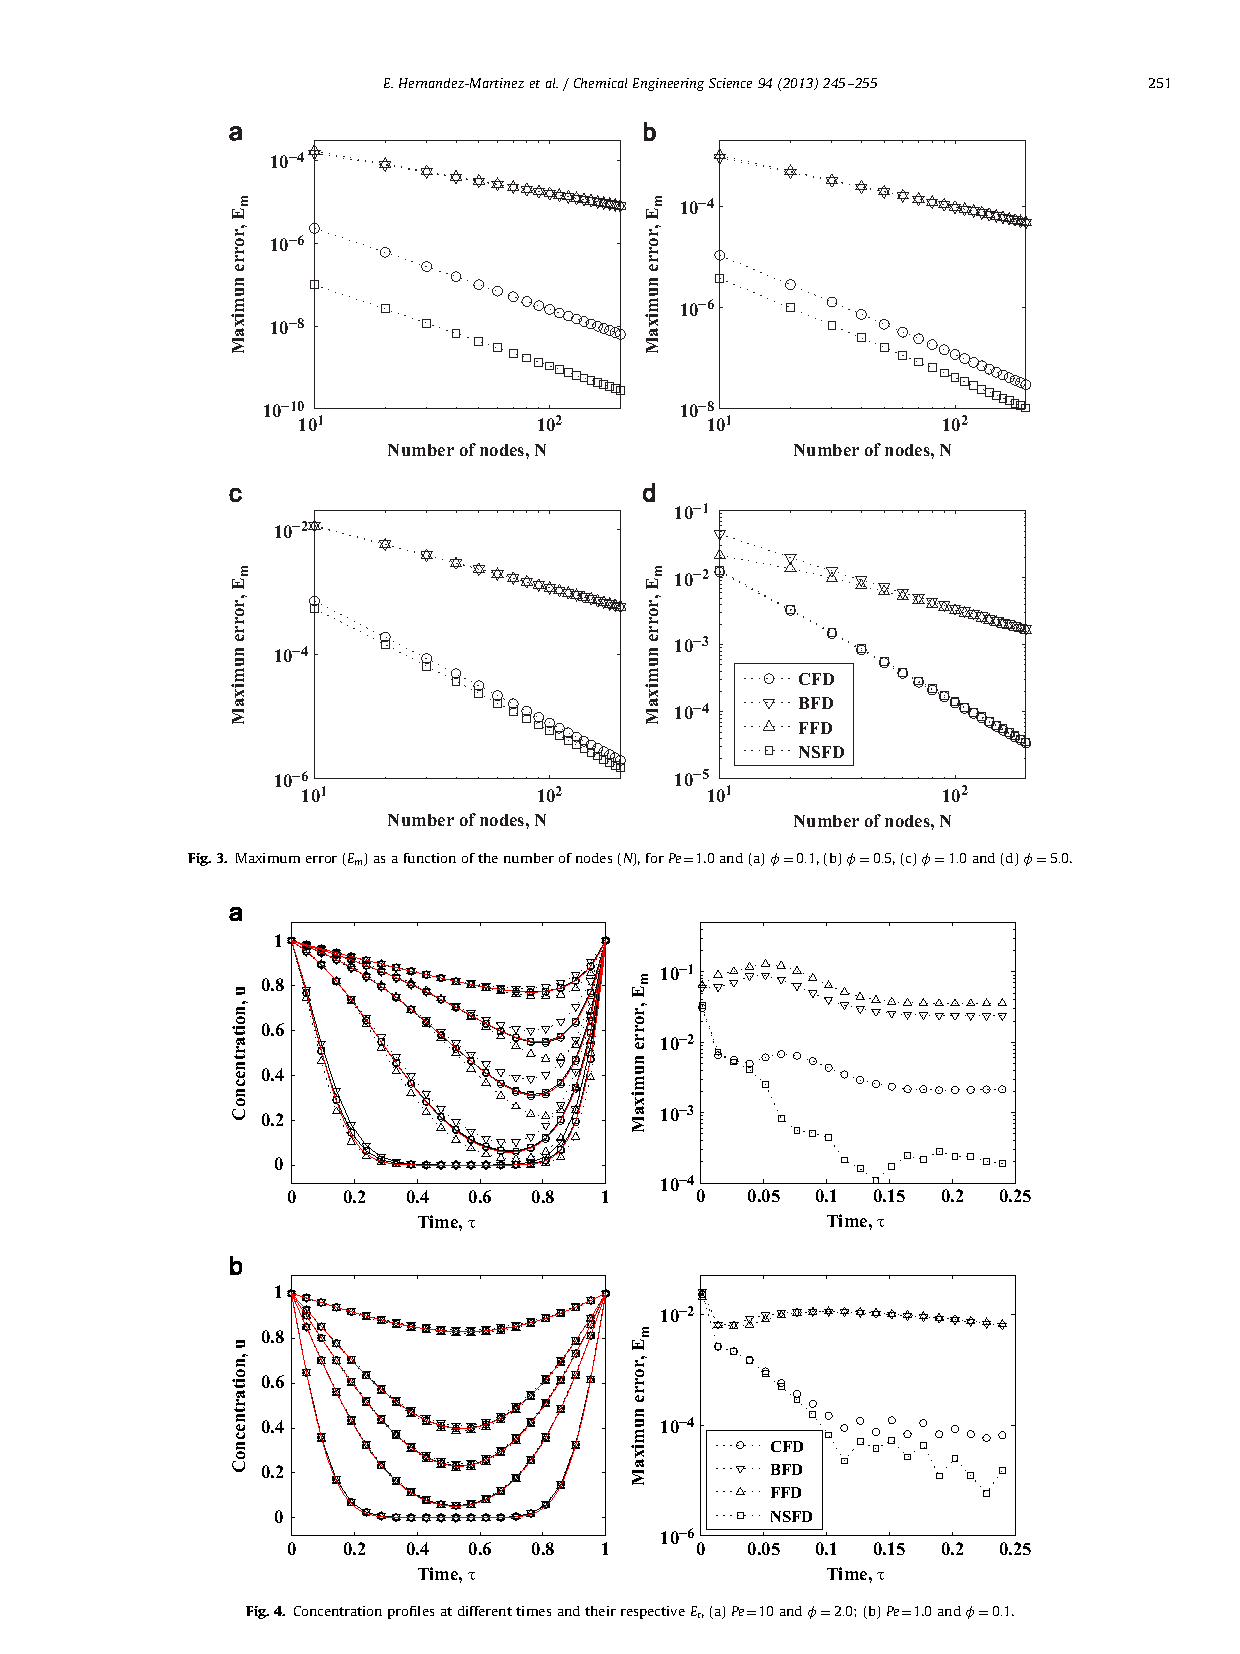
\includegraphics[trim=80 45 80 420,clip]{./pic/f3.pdf}
\caption{当$Pe=1.0$时最大误差($E_m$)与节点数$N$的关系}\label{fig:4}
\end{figure}
\subsection{轴向扩散的管式反应器}
作为第二个例子,我们考虑一个轴向扩散的管式反应器.这个模型的物质和能量平衡方程可以表述为相关的非线性抛物线PDE方程.它的无维度
形式如下:
\begin{multline}\label{eq:27}
 \dfrac{\partial y(\xi,t)}{\partial t} = \dfrac{1}{Pe_y}\dfrac{\partial^2 y(\xi,t)}{\partial \xi^2}
 -\dfrac{\partial y}{\partial \xi} \\
 +BDa(1-z(\xi,t))\exp\left(\dfrac{y(\xi,t)}{1-y(\xi,t)/\lambda}\right)-\sigma(y(\xi,t)-y_j)
\end{multline}
\begin{equation}\label{eq:28}
 \dfrac{\partial z(\xi,t)}{\partial t}=\dfrac{1}{Pe_z}\dfrac{\partial^2 z(\xi,t)}{\partial xi^2}
 -\dfrac{\partial z}{\partial \xi}+BDa(1-z(\xi,t))\exp\left(\dfrac{y(\xi,t)}{1-y(\xi,t)/\lambda}\right)
\end{equation}
边界条件为
\begin{align*}
\left.\dfrac{\partial y(\xi,t)}{\partial \xi}\right|_{\xi=0}&=Pe_yy(t,0), & \left.\dfrac{\partial z(\xi,t)}{\partial \xi}\right|_{\xi=0}&=Pe_zy(t,0)\\
\left.\dfrac{\partial y(\xi,t)}{\partial \xi}\right|_{\xi=1}&=0, & \left.\dfrac{\partial z(\xi,t)}{\partial \xi}\right|_{\xi=1}&=0
\end{align*}
初值条件为
\begin{equation*}
 y(\xi,0)=0 \qquad z(\xi,0)=0
\end{equation*}
其中,~$y(\xi,t)$和$z(\xi,t)$是无量纲的温度和浓度值.相应地,~$Da$是Damkohler系数,~$Pe_y$和$Pe_z$是物质和热量传递的Peclet常数.
$\delta$是一个无量纲的热传导系数,~$B$是无量纲的绝热升温,~$\lambda$是无量纲的活化能.根据模型参数的值,温度特性可以产生很多
种类的变化.表~\ref{tab:1}~说明了这样的一组参数.图~\ref{fig:5}~说明了这样的参数对应的分布.在数值分析上,我们强调物理参数
对浓度分布的影响,即当$Da$的数值较大时,过程主要由化学反应主导而当$Da$较小时,过程主要由传递现象主导.另一方面,如果$Pe\rightarrow0$
时,传递现象由扩散主导.当$Pe\rightarrow \infty$时传递现象由对流现象主导.
\begin{table}[hbtp]
\caption{不同管式反应器的参数\label{tab:1}}
% \begin{tabular*}{\textwidth}{@{\extracolsep{2.8cm}}cD{.}{.}{3}D{.}{.}{3}D{.}{.}{3}}
\begin{tabularx}{\textwidth}{XXXX}
\toprule
参数  	  &  (a)	&  (b) 		 &  (c)   	\\
\midrule
$Pe_y$    &  5.0	&  5.0		 &  5.0	 	\\
$Pe_z$	  &  5.0        &  5.0  	 &  5.0   	\\
$\lambda$ &  20.0	&  20.0 	 &  20.0	\\
$B$	  &  11.0	&  5.0		 &  14.0	\\
$Da$	  &  0.174	&  0.875	 &  0.185	\\
$\sigma$  &  2.25	&  5.0		 &  3.0		\\
$y_j$	  &  0.1	&  0.1		 &  0.0		\\
\bottomrule
\end{tabularx}
\end{table}
\subsubsection{基于格林函数的NSFD格式}
不同于方程~\ref{eq:1}~中Peclet系数与对流系数相乘,在管式反应器模型中Peclet系数的相反数与传导和对流系数是相乘的.
为了简化模型的建立,我们考虑令$Pe_y=Pe_z=Pe$.即共轭运算即为$L=\frac{\partial}{\partial x}[(\exp(-Pex)/Pe)(\partial
/\partial x)]$.因此,积分形式及格林函数为
\begin{equation}
 u(x,t)=\dfrac{\exp(-Pea)}{Pe}\dfrac{\partial G(a,x)}{\partial z}\dfrac{\gamma_a}{\beta_a}-
        \dfrac{\exp(-Peb)}{Pe}\dfrac{\partial G(b,x)}{\partial z}\dfrac{\gamma_b}{\beta_b}
\end{equation}
\begin{equation}
G(z,x)=\dfrac{1}{G^*}\begin{cases}
        [\exp(Pez)-\exp(Pea)k_a][\exp(Pex)-\exp(Peb)k_b]	&	z<x	\\
        [\exp(Pez)-\exp(Peb)k_b][\exp(Pex)-\exp(Pea)k_a]	&	z\geq x	
       \end{cases}
\end{equation}
其中,$G^*=[\exp(Peb)k_b-\exp(Pea)k_a]$.根据方程~\ref{eq:14}--\ref{eq:19}~中所列的步骤,得到NSFD差分格式是很容易的,即
\begin{equation}
 \begin{aligned}
  \dfrac{\dif u_1(t)}{\dif t} &= \dfrac{a_1\dfrac{\gamma_a}{\beta_a}-b_1 u_1(t)+c_1 u_2(t)}{Pe}-R(u_1(t))\\
  \dfrac{\dif u_i(t)}{\dif t} &= \dfrac{a_iu_{i-1}(t)-b_iu_i(t)+c_iu_{i+1}(t)}{Pe}-R(u_i(t))\\
  \dfrac{\dif u_N(t)}{\dif t} &= \dfrac{a_Nu_{N-1}(t)-b_Nu_N(t)+c_N\dfrac{\gamma_b}{\beta_b}}{Pe}-R(u_N(t))
 \end{aligned}
\end{equation}
其中,$a_i$,$b_i$,$c_i$是在方程~\ref{eq:20}~中给出的.
\begin{figure}
\centering
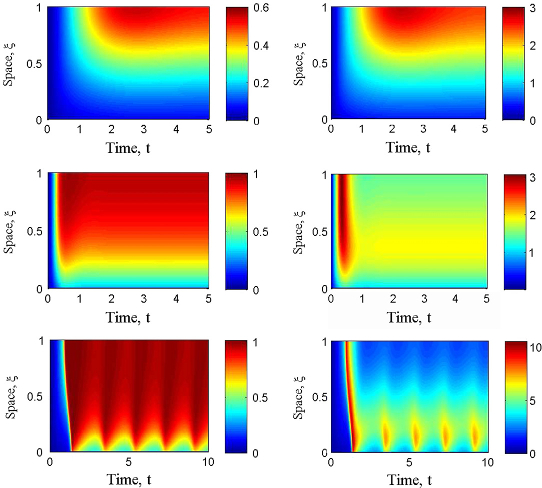
\includegraphics[scale=0.7]{./pic/f5.jpg}
\caption{管式反应器的浓度和温度的分布情况}\label{fig:5}
\end{figure}
\begin{table}
\caption{解管式反应器稳态模型的CPU时间(秒)\label{tab:2}}
\begin{tabularx}{\textwidth}{@{\extracolsep{5mm}}*{6}{X}}
\toprule
\multicolumn{3}{l}{(a)}&\multicolumn{3}{l}{(b)}\\
\cmidrule{1-3}\cmidrule{4-6}
Pe 	&	NSFD	&	CFD	&	Da	&	NSFD	&	CFD \\	
\midrule
0.01	&   14.352	&	12.729	&	0.01	&	8.408	&	7.347	\\
0.05	&   14.008	&	11.749	&	0.05	&	7.051	&	7.815	\\
0.1	&   13.603	&	11.715	&	0.1	&	10.795	&	7.971	\\
0.5	&   13.854	&	11.512	&	0.5	&	12.495	&	10.436	\\
1.0	&   14.118	&	11.965	&	1.0	&	16.146	&	12.963	\\
5.0	&   15.865	&	13.135	&	5.0	&	56.846	&	48.235	\\
10.0	&   15.631	&	12.745	&	10.0	&	23.150	&	19.681	\\
50.0	&   16.161	&	12.776	&	50.0	&	155.002	&	140.68	\\
100.0	&   17.113	&	13.228	&	100.0	&	121.896	&	107.749	\\
\bottomrule
\end{tabularx}
\end{table}
\begin{figure}
\centering
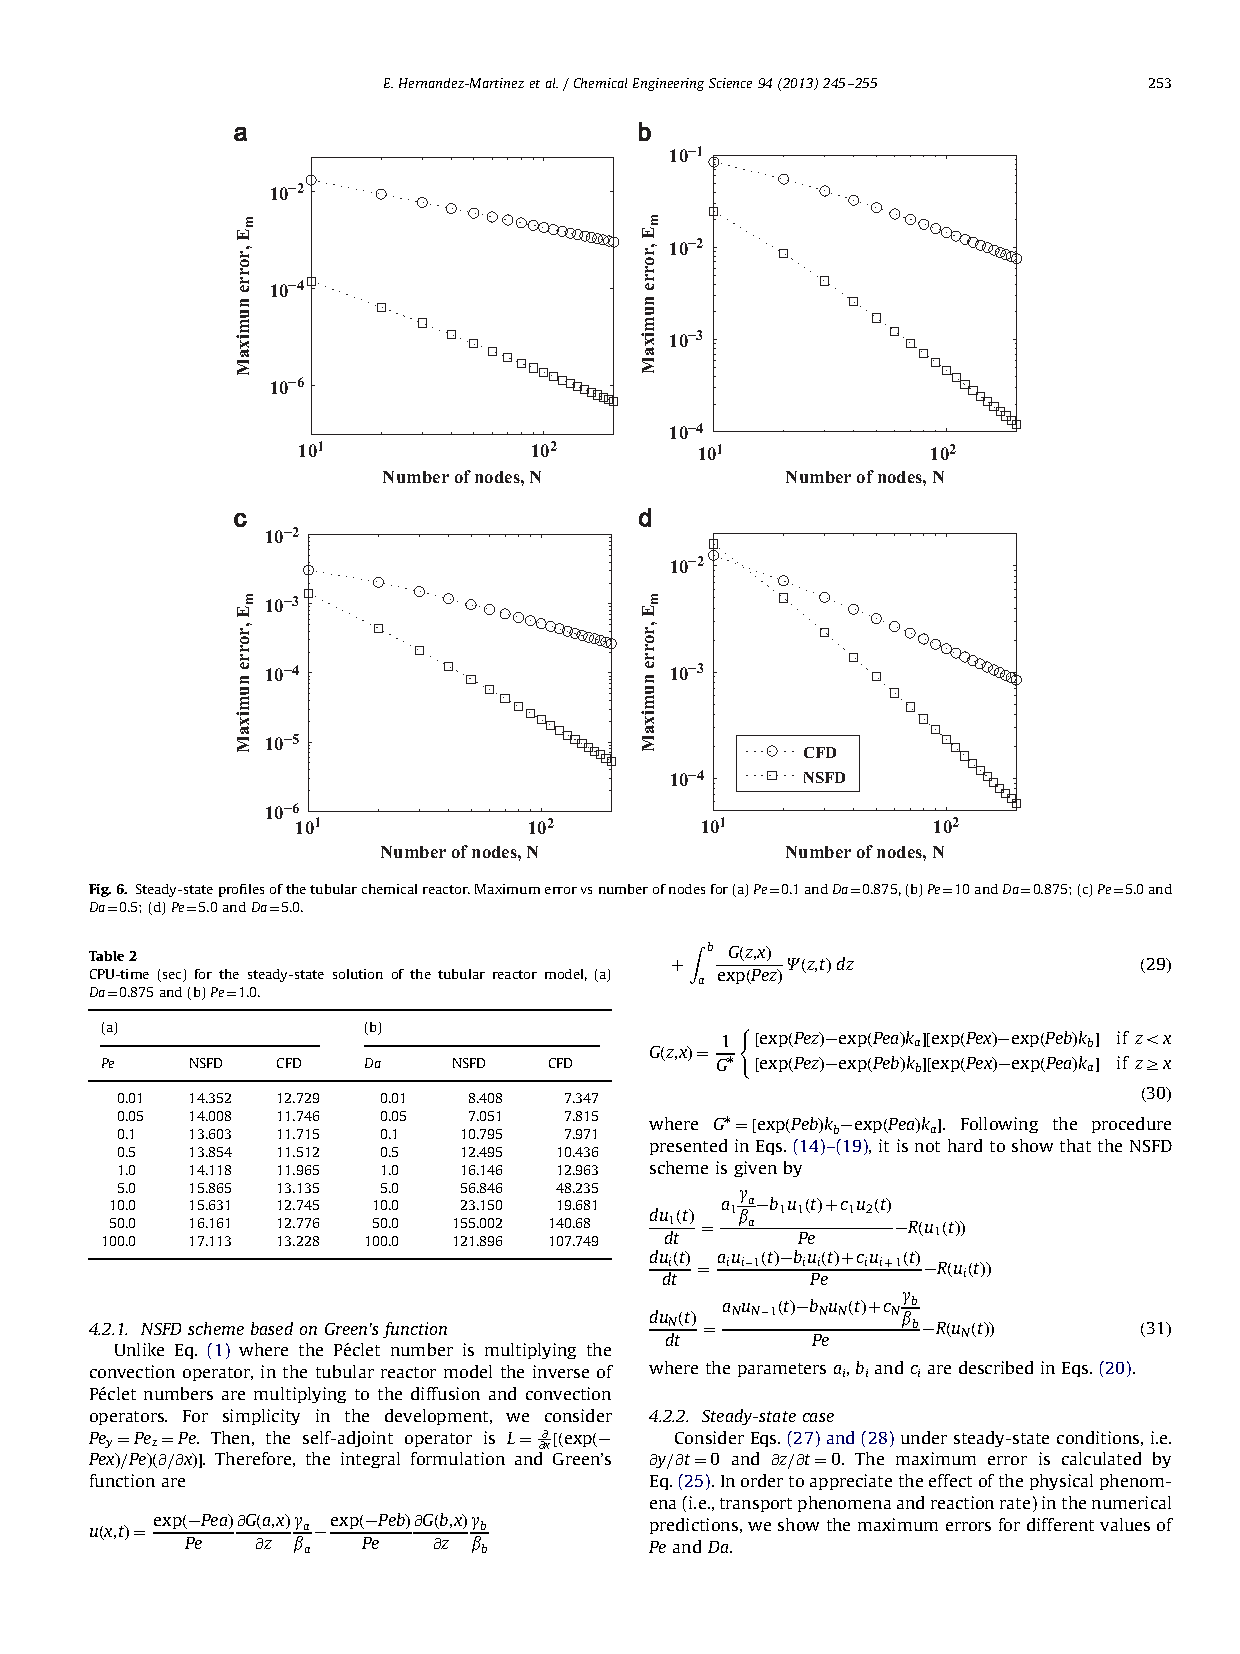
\includegraphics[trim=80 390 80 60,clip]{./pic/f6.pdf}
\caption{管式反应器的稳态特性}\label{fig:6}
\end{figure}
\subsubsection{稳态}
考虑方程~\ref{eq:27}~和方程~\ref{eq:28}~在稳态下的条件,即$\partial y/\partial t=0,\partial z/\partial t$.
最大的误差是由方程~\ref{eq:25}~引起的.为了表现物理现象在数值预测上的效果,我们给出了不同$Pe$和$Da$值下的最大误差.\par
考虑与相应的热点地区的现象的一组参数,图~\ref{fig:6}~表示NSFD格式的表现要优于CFD差分格式.在扩散现象占优的过程中,我们
可以观察到NSFD具有很好的表现.\par
另一方面,表~\ref{tab:2}~中列举了在不同条件下求解管式反应器数值解所需要的CPU时间.我们采用得到10--100节点,其中有10个空白
节点的平均时间来计算CPU时间.为了观察到反应和传递现象各自需要的CPU时间,我们采用了不同的Damkohler数和Peclet数.
一般地,传统的中心差分格式比NSFD差分格式要节省计算资源,这是因为$\alpha$,$\beta$,$\gamma$都是指数函数,这些函数需要更多的
计算机时间去计算.尽管如此,NSFD具有$O(h^2)$阶次下可以接受的CPU时间.
\subsubsection{动态}
我们采用2000个节点的由\texttt{COMSOL}得到的数值结果作为参考解.我们采用4/5阶的Runge-Kutta法(MATLAB中的
\texttt{ode45}包)和参数$\delta t = 0.01$来求解微分方程的积分.为了比较格林函数的NSFD格式的性能表现,图
~\ref{fig:7}~表现了$N=100$时的温度和浓度特性,这样可以观察热点的动态变化并与参考解进行比较.然而,
NSFD格式与\texttt{COMSOL}的结果相一致,都比CFD的结果要优.这个结果说明基于积分定律的NSFD是一个很好的替代方法
去解复杂的数学模型.为了估计计算时间,我们考察了当$N=200$和$N=50$时$Da$和$Pe$的值.在这种情况下,NSFD格式要
更加节省CPU时间.总体来说,NSFD格式是一个较好的替代方法来解对流扩撒反应方程.
\begin{figure}[t]
\centering
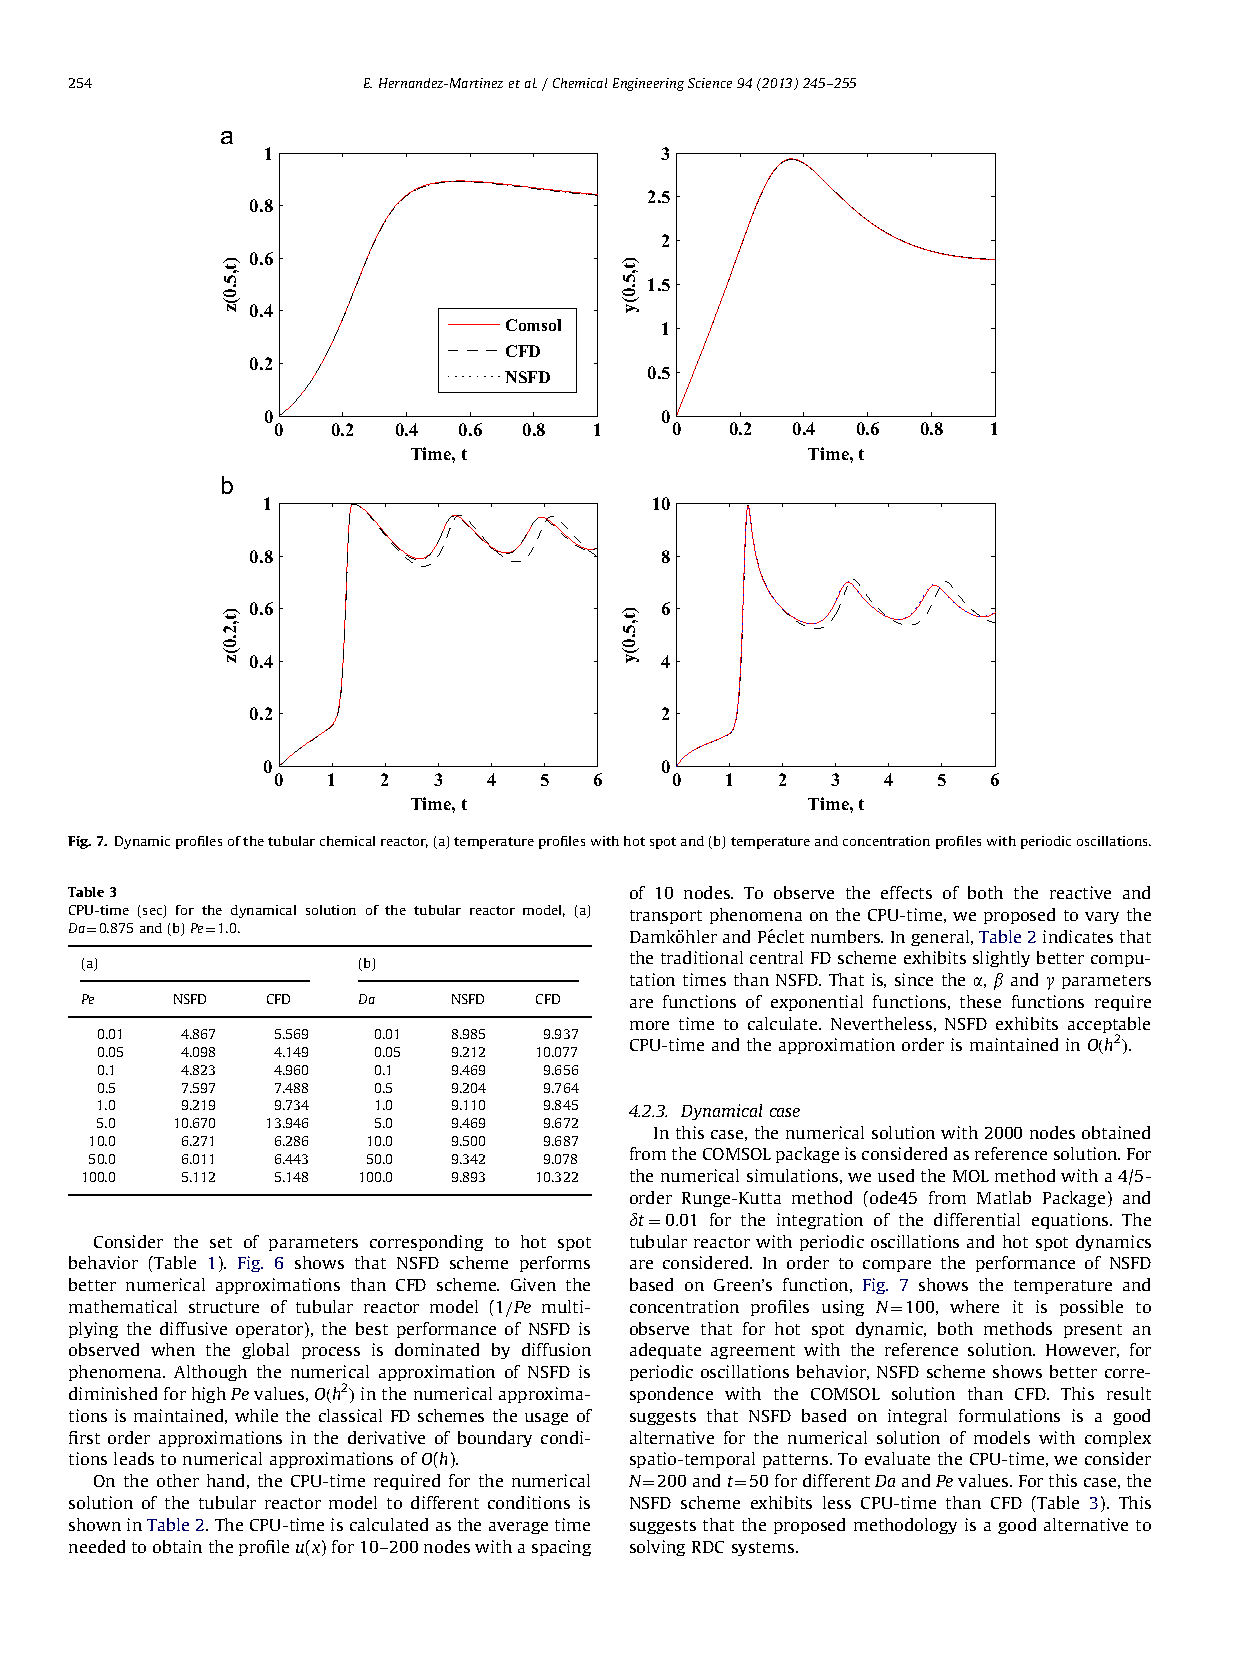
\includegraphics[trim=80 400 80 60,clip]{./pic/f7.pdf}
\caption{管式反应器的动态特性}\label{fig:7}
\end{figure}
\section{结论}
在这篇文章中,我们论证了基于格林函数的NSFD有限差分格式在解通常边界条件的非线性对流扩散反应方程系统中的应用.
通过使用这种方法,可以得到自然的$O(h^2)$的近似而与其他规则无关.总的来说,格林函数已经变成了常用的框架来处理
包括传统的和非标准的FD格式,避免了泰勒展开.在这种方法中,我们的方法可以在更多的系统上得到拓展和应用.同时,在准确度
分析中,比照标准的FD格式我们的方法也占有优势.
\end{document}